%
% Name: Accelerating Multi-dimensional Search Mid-Project Report
% Author: Donald Whyte (sc10dw@leeds.ac.uk)
%

\documentclass[notitlepage]{article}

\usepackage[margin=2.5cm]{geometry} % easy page formatting
	\geometry{letterpaper}
\usepackage{doc} %special logo commands
\usepackage{url} % formatting URLs
\usepackage{datetime} % up-to-date, automatically generated times
\usepackage{amsmath}
\usepackage{amsfonts}
\usepackage{multirow}
% For graphic files
\usepackage{graphicx}
\usepackage{epstopdf}
\DeclareGraphicsRule{.tif}{png}{.png}{`convert #1 `dirname #1`/`basename #1 .tif`.png}

\usepackage{algorithm}
\usepackage{algorithmic}

\usepackage{pdflscape}
\usepackage{rotating}
\usepackage{wrapfig}

\usepackage{cite} 

\usepackage{caption}

\usepackage{fancyhdr}
\chead{Donald Whyte}
\lhead{}
\rhead{}


\title{Accelerating Multi-dimensional Search \\ Mid-Project Report}
\author{Donald Whyte}
\date{\today}

\pagestyle{fancy} % so header appears on each page

\begin{document}

\null  % Empty line
\nointerlineskip  % No skip for prev line
\vfill
\let\snewpage \newpage
\let\newpage \relax
\maketitle
\let \newpage \snewpage
\vfill 
\break % page break

\tableofcontents

\vspace{4em}

\section{Introduction}
	\chapter{Introduction}
\label{chap:introduction}
\centerline{\rule{149mm}{.02in}}
\vspace{2cm}

\section{Problem Definition}

TODO

\section{Aims}

TODO

\section{Objectives}

TODO

\section{Minimum Requirements}

TODO

\section{Extended Requirements}

TODO

\section{Deliverables}

TODO

\section{Evaluation Criteria}

TODO

	\subsection{Aim}

This project will survey existing multi-dimensional search structures which attempt to solve the multi-dimensional search problem, identifying the major challenges of the field and how this has guided the development of structures throughout the last two decades. The core aim of the project is to implement one or more modern index structures, optimising them specifically for high-dimensional datasets. These implementation(s) will be then be evaluated with respect to their proposed performance in the literature and pre-defined baselines using test datasets. This evaluation will highlight the found performance bottlenecks in the implementations and limitations of the algorithms themselves.

	\subsection{Objectives}

The objectives of the project are:
\begin{itemize}
	\item Understand the current state and challenges of the field of multi-dimensional search
	\item Implement multi-dimensional search structures
	\item Perform performance analysis on implementations and attempt to optimise structures for greater performance on high-dimensional data
	\item Evaluate and compare performance of final structures to pre-defined baselines, unoptimised structures and their reported performance in the literature
\end{itemize}

	\subsection{Requirements}

The minimum requirements are closely related to the objectives of the project. They are:
\begin{enumerate}
	\item Produce literature review describing the current state of multi-dimensional search structures, comparing their strengths and weaknesses and highlighting core challenges of the field
	\item Implement at least one index structure and perform performance analysis of the implementation
	\item Perform one set of modifications to the implemented structure in an attempt to optimise its performance
	\item Evaluate and compare performance of final implementations to pre-defined baselines, unoptimised structures and their reported performance in the literature
\end{enumerate}

Possible extensions of the project include:
\begin{enumerate}
	\item Parallelising implementations using technologies such as Haskell, CUDA (GPGPU) or MPI
	\item Developing an entirely new index structure, which is also implemented and evaluated
\end{enumerate}

\subsection{Deliverables}

The following will be delivered upon project completion:
\begin{enumerate}
	\item Documented source code of implemented index structures
	\item User manual describing how to use the index structures
	\item Evaluation of the performance of the implemented index structures, with respect to pre-specified test data
	\item Generated synthetic data that is used for the evaluation
\end{enumerate}

\subsection{Core Assumptions}
\label{sec:core-assumptions}

Throughout the project, some assumptions have been made. These are used to narrow the scope of the project and allow more time to be spent focusing on the core aim of the project (high-dimensional data). The assumptions are:
\begin{enumerate}
	\item Datasets have a ``high" number of dimensions ($\geq 10$), meaning the performance of the index structures will be measured using data with at least 10 dimensions. However, data using a smaller number of dimensions may be used for the purposes of understanding how the implementations behave with respect to dimensionality.
	\item Datasets will be able to fit into the main memory (i.e. RAM) of the machine used for evaluation. That is, none of the data is paged to secondary memory and page accesses causing reduced performance does not need to be considered.
	\item Datasets are dynamic, meaning points may be inserted, deleted or updated at any time.
\end{enumerate}
Furthermore, the project is focused on the \textit{geometric} applications of multi-dimensional search and not databases. This is the primary reason assumption (2) has been made.

No assumptions have been made about the distribution of data. This means the implementations' performance will be evaluated using a variety of distributions.

\section{Methodology}
	\chapter{Methodology}
\label{chap:methodology}
\centerline{\rule{149mm}{.02in}}
\vspace{2cm}

\section{TODO}

TODO

	\subsection{Schedule}
\label{sec:schedule}

The original schedule was devised near the end of the first week of the project, on 31/01/14. The schedule was broken down into the individual tasks required to complete the defined milestones. These tasks were then grouped into different \textbf{phases}, which run sequentially (with some in parallel). The phases of the project and their milestones are:
\begin{enumerate}
	\item ``Project Definition""
	\begin{itemize}
		\item \textbf{Project Outline Defined} -- defined outline of project's aims and objects
	\end{itemize}
	\item ``Literature Review and Data Collection"
	\begin{itemize}	
		\item \textbf{Literature Review Complete} -- produced literature review of multi-dimensional search
		\item \textbf{Data Collected} --  decided and collected non-synthetic external test data sets
	\end{itemize}
	\item ``Initial Implementation"
	\begin{itemize}	
		\item \textbf{Software Deliverables Decided} -- determined index structures to implement and the technologies to use
		\item \textbf{Initial Implementation Finished} -- completed initial, unoptimised implementations of chosen index structure(s)
	\end{itemize}
	\item ``Mid-project Presentation and Report"
	\begin{itemize}	
		\item \textbf{Mid-project Presentation Delivered} -- delivered mid-project presentation to relevant research group
		\item \textbf{Mid-project Report Finished} -- submitted mid-project report
	\end{itemize}	
	\item ``Performance Tuning"
	\begin{itemize}
		\item \textbf{Software Deliverables Finished} -- produced final, optimised implementations of the index structure(s), which is ready for a final evaluation
	\end{itemize}
	\item ``Final Report Write-up"
	\begin{itemize}
		\item \textbf{Final Report Finished} -- submitted write-up of the final report
	\end{itemize}
	\item ``Student Symposium"
	\begin{itemize}
		\item \textbf{Final Presentation Delivered} -- delivered final project presentation
	\end{itemize}
\end{enumerate}

The performance tests and evaluation of the initial implementation could produce unexpected results, showing that it may be beneficial to implement an entirely different index structure or use a different technology. Therefore, deciding on a \textit{fixed} set of index structures to implement  would be unwise. Doing means there is no way to go backwards and revise the project plan if performance tests highlight a poor index structure or technology. As such, a decision has been made on a \textit{single, initial} index structure to implement. This will be evaluated and based on that evaluation, it will be optimised or it will be discarded in favour of another index structure. This will be repeated in iterations, where each iteration contains the following sub-phases:
\begin{enumerate}
	\item \textbf{Design} -- plan exactly what needs to be done in the iteration and the architectural design of the system/implementation
	\item \textbf{Build} -- implement an index structure or perform one or more optimisations
	\item \textbf{Test} -- perform correctness tests on index structure to ensure it (still) works
	\item \textbf{Performance Analysis} -- perform performance analysis on index structure developed/optimised
	\item \textbf{Evaluation} -- evaluate the produced results and use it to decide what to implement or optimise in the next iteration
\end{enumerate}
When enough iterations have passed or there is no time left to spend on the Design and Implementation phase, the iterations will stop, with the evaluation of the optimised structure(s) in last phase being the final evaluation that is used in the Final Report Write-up phase. This iterative approach is illustrated in the full project process diagram shown in Figure \ref{fig:full-project-process} in the appendix.

Figure \ref{fig:initial-schedule} and Figure \ref{fig:initial-milestone-timeline} show a Gantt chart of the phases and a timeline annotated with the project's milestones respectively. Due to the often uncertain nature of research projects, especially when one does not have much knowledge of the relevant field prior to the project, it was decided that the schedule will \textit{not} break down each phase into fine-grained sub-tasks. This is to avoid the likely situation of some of the tasks taken longer than others and having the project greatly trail away the original schedule, to the point where it's not used. Instead, these higher level phases and milestones will guide development, following the process shown in Figure \ref{fig:full-project-process}.

The plan has changed since its initial conception. The original plan stated that the initial, unoptimised implementations of the index structures should be finished before the mid-project presentation or report. The idea behind this decision was that having implementations of index structures finished before the presentation, an initial evaluation of the index structures could be performed. The results from this evaluation could then used in the presentation and report as justification for project decisions. However, due to the scope of the research field, the literature take one more week than expected. This meant that there was little time between the end of the literature review and the start of the mid-project presentation and report.

Furthermore, additional time was required to determine the nature of the data that to be used for evaluation. This knowledge informs the decisions on which index structures to implement, so it was felt that rushing into implementation may result in a poor decision on which structures to implement. Therefore, implementation has been pushed back until after the submission of the mid-project report. By doing this, there is more time to collect the research findings and make a more informed decision on the index structure to implement.

Figure \ref{fig:revised-schedule} and Figure \ref{fig:revised-milestone-timeline} show a Gantt chart of the revised phases and a timeline marked with the new milestones. The date this report has been submitted is also marked on the Gantt chart, showing what phases and milestones are left to complete before the end of the project. With the new schedule, the ``Initial Implementation" phase has been removed and the ``Performance Tuning" phase has changed to ``Design and Implementation". As a consequence, the milestones \textbf{Software Deliverables Decided} and \textbf{Initial Implementations Finished} have been removed. The \textbf{Software Deliverables Finished} milestone remains, but now marks the end of ``Design and Implementation" phase.

``Design and Implementation" encompasses the design, implementation and evaluation of the index structure. This will contain multiple iterations of the implementation process described previously. An unoptimised, functional implementation is the barest deliverable required to perform the final evaluation. To ensure this is developed, the \textbf{Initial Implementation of Software Deliverables Complete} milestone has been created. The first iteration of ``Design and Implementation" will be two weeks and will be used to develop the baselines and initial implementation of the chosen index structure. \textbf{Initial Implementation of Software Deliverables Complete} should be met at the end of this first iteration. Subsequent iterations will last a week to coincide with the weekly supervisor meetings, which will be at the start of each iteration. 

	\subsection{Technology}

\subsubsection{Programming Language}

There exist many programming languages, all developed for specific purposes. Three programming languages have been considered for this project, with each having different properties. This section will describe these languaes, discuss their differences and state which will be used for this project and why.

\textbf{Python} is a high-level interpreted language built for general-purpose computing, which has a large standard library and many third-party libraries \cite{python}. \textbf{C++} is a middle-level, compiled systems programming language, combining low-level features (e.g. manual memory management) and high-level features (e.g. object-orientated programming) \cite{cpp}. C++ applications are compiled straight to the native machine's CPU instruction set, meaning less time is spent translating the code to instructions the hardware can directly execute. \textbf{Haskell} is a purely functional general-purpose programming language which compiles to a native executable, similar to C++ \cite{haskell}. Being purely functional means that applications written in Haskell have no mutable state. This is unlike Python and C++, whose applications have mutable state (since both languages are imperative).

The following aspects have been considered when deciding which language to use:
\begin{itemize}
	\item \textbf{Performance} -- how fast the final application can run. This is based on a number of factors, such as how many intermediary layers there are between the code and the physical machine. Higher-level languages require the computer to do more work, as it has to convert the application's instructions into CPU instructions that are executed directly on the processor.
	\item \textbf{Ease/Speed of Development} -- this encompasses multiple aspects of a language. In order to develop applications quickly, the language must have a mature tool set, large amounts of documentation and support, be easy to understand and require little boilerplate code (so less time is required to write the code). This makes it easier for the developer to write the application, increasing the speed it can be developed.
	\item \textbf{Portability} -- can an application written in a given language execute on many supported platforms or just one? Do multiple versions of the application have to be written or compiled for each platform?
\end{itemize}
 
Executing a Python statement often has more overhead than it would for C++ or Haskell. This is because Python is a high-level, interpreted language, where statements are compiled into bytecode at runtime which is then run on a virtual machine (which translates the bytecode to native assembly instructions). Therefore, many Python applications run slower than C++ or Haskell, which pre-compile applications to native CPU instructions. However, due to the large amount of experience I have in Python, its large standard library and the higher number of abstractions, Python would most likely result in the fastest development time. 

Haskell's pure functional nature makes it fundamentally different than most popular languages and I also have little experience writing programs in a purely functional style. It is predicted this will increase the time it takes to develop the structures, as there is more overhead in learning about functional programming. However, if it is decided that the index structures will be parallelised, then the lack of state and built-in support for parallelisation \cite{parallel-haskell} would make Haskell a powerful choice.

Despite speed of development being important, the primary aim of the project is the acceleration of search. Haskell can be used to write highly optimised code, especially when implementing parallel algorithms to utilise multiple CPU cores. C++ gives the developer more control over the computation and management of memory, allowing for low-level performance tuning. The trade-off for this control is the added complexity of the language \cite{cpp-hard}, leading to an increased amount of code to write and the decrease in development speed that follows. However, C++ is also a mature language with a large set of tools and resources to aid development. Additionally, I have significantly more experience developing in C++ than Haskell. It is unlikely I would be able to produce well-written, optimised Haskell code to fine-tune performance in such a short time. Therefore, C++ has been chosen as the language to use for developing the initial implementation of the index structure.

\subsubsection{Development Tools}
\label{sec:development-tools}

Various tools will be used throughout the development of the structures. \textbf{CMake} \cite{cmake} will be used to automate the building of the written C++ programs. Using a build automation tool means a Makefile can be automatically generated by writing simpler, higher-level and cross-platform scripts, meaning less time is spent focused on build scripts.

Unit tests will be written to ensure the implemented index structures and all the associated algorithms are functioning correctly. A unit test ensures a single unit of the code is exhibiting the desired behaviour. A test is performed in isolation, preventing other code in the application from being executed so it does interfere with the test's results \cite{automated-defect-prevention}. A unit test framework is a suite of code and tools that make writing unit tests easier and faster \cite{unit-test-frameworks}. C++ has many unit testing frameworks, such as CppUnit \cite{cppunit}, NullUnit \cite{nullunit} and Google Test \cite{google-test}. \textbf{Google Test} has been chosen for this project because of the wide feature set and the comprehensive documentation available (at \cite{google-test}).

Version control is a way of tracking changes to textual documents, as well as \textit{who} made the changes \cite{pragmatic-version-control}. A VCS (version control system) will be used to track the changes of the implementation's source code, tests and built automation scripts. Despite this project only having a single developer, there are multiple reasons it has been decided to manage the source code using a VCS. Firstly, it allows the developer to easily keep a log of the changes made to any file and \textit{why} those changes were made. One can also revert source files to prior versions if bugs are found or previously deleted code is required again, Finally, using a VCS means there will be multiple copies of the source code, which can be used as backups to mitigate the damage caused by data loss. The distributed VCS \textbf{Git} \cite{git} will be used for this project, due to the developer having prior experience in the tool, meaning less time is taken from implementation to learn a new tool.

\subsubsection{Performance Analysis Tools}

In addition to considering the theoretical performance of the chosen algorithms, the implementations' performance will be tested using profiling. Profiling is a way of measuring the performance of a program or system \cite{efficient-cpp} and is used to provide insight into which parts of the code take the longest or use the most memory (i.e. where the performance bottlenecks are). A profiler is a tool which measures some performance metrics of a program. Since the core goal of this project is accelerating multi-dimensional search, being able to measure the performance of the implementations and identify where the performance bottlenecks are is incredibly useful.

To perform the evaluation (see Section \ref{sec:evaluation}), a profiler that can measure heap usage and cache misses will be used. One which can produce call graphs with timings, that measure the flow of execution and how much time is spent in each function, is also desired. Using a profiler that produces little slow down is useful, but not critical, since timings could be scaled to take the extra overhead into consideration. 

Many profilers were considered when choosing one for this project. Intel VTune \cite{intel-vtune} is feature-rich profiler for Intel-based machines, but it is proprietary, so it will not be used for this project. Valgrind \cite{valgrind}, Profiny \cite{profiny} and gperftools \cite{gperftools} are freely available profilers. Out of these, only Valgrind can measure both heap usage and cache misses. gperftools can generate a visualisation of program flow and where the program spends most of its time via a call graph image, with just a single command. gperftools provides a similar feature for heap profiling as well. Therefore, both Valgrind and gperftools will be used for profiling.

\section{Progress Report}

Referring to the schedule defined in Section \ref{sec:schedule}, as of the submission of this report, the following phases are complete: ``Project Definition", ``Literature Review and Data Collection" and ``Mid-project Presentation and Report". The following milestones have also been met: \textbf{Project Outline Defined}, \textbf{Literature Review Complete},  \textbf{Test Data Collected}, \textbf{Mid-project Presentation Delivered} and \textbf{Mid-project Report Finished}. 

This means that the project's aims, objectives and requirements have been defined, with a clear description on what the final deliverables are. Extensive research has been performed on the multi-dimensional search problem, existing solutions, their limitations and general challenges the field faces. All this information was written up into a stand-alone literature review document that has been integrated into Section \ref{sec:background-research} of this report. Which index structure to implement initially has been determined and the technologies to use to develop the implementation have also been decided. The development process has been determined which, as discussed in Section \ref{sec:schedule}, will involve multiple iterations of implementation, testing and evaluation. Finally, a presentation has been performed to the relevant research group, Computational Science and Engineering, outlining the project's aims, current progress and the design, implementation and evaluation approach which will be taken throughout the next two months.

See Section \ref{sec:next-steps} for what actions will be performed next, after the submission of this report.

\chapter{Background Research}
\label{chap:background_research}
\centerline{\rule{149mm}{.02in}}
\vspace{2cm}

This chapter contains a literature review on multi-dimensional search. First, the problem will be formally defined. Then, the field's core challenges and their implications will be summarised. Existing solutions (index structures) which perform multi-dimensional search will be described, highlighting their limitations with respect to the core challenges. Finally, a discussion on how to choose a structure to a given problem and existing work on parallelising search will be given.

\section{Formal Problem Definition}
\label{sec:definition}

We define \textbf{data space} as the space containing all possible data items for some domain. Let $d$ be the number of dimensions in this data space. The universe of the space is defined as $[min,max]^d$, where $min$ is the minimum possible value and $max$ is the maximum possible value, such that $min \leq max$. All values are real numbers. Every data item is typically represented as a point $p \in [min,max]^d$. Figure \ref{fig:data-space} shows an example of a 2D space ($d = 2$), where $min = 0$ and $max = 1$. This means all possible data items within the data space are represented as a point in the universe $[0, 1]^2$.

A \textbf{multi-dimensional search structure}, often referred to as an \textbf{index structure}\footnote{this will be used to refer to such structures throughout the rest of this document} \cite{r-tree-variants}, is a data structure which stores data items in a way which allows operations and queries to be performed quickly \cite{dynamic-data-structures}. These structures can be \textbf{static} or \textbf{dynamic}. Static index structures are built for a specific set of points which never change. Dynamic index structures support changing data, and provide mechanisms for adding, deleting or updating (i.e. moving) a point. These structures typically have some form of balancing procedure \cite{dynamic-data-structures} that maintains certain properties which allow for fast queries. The three core operations supported by dynamic index structures are:
\begin{itemize}
	\item \texttt{insert} -- insert a new point into the structure
	\item \texttt{delete} -- delete a point already contained within the structure
	\item \texttt{update} -- change location (i.e. one or more attributes) of an existing data item
\end{itemize}
Some dynamic structures have a \textbf{build stage} when then structure is initially created, which provide fast ways of pre-loading data \cite{pyramid-tree}. Otherwise, an index structure can be incrementally created by repeatedly using the \texttt{insert} operation for each item in the set.

\begin{wrapfigure}[12]{r}{0.4\textwidth}
	\vspace{-40pt}
	\begin{center}
		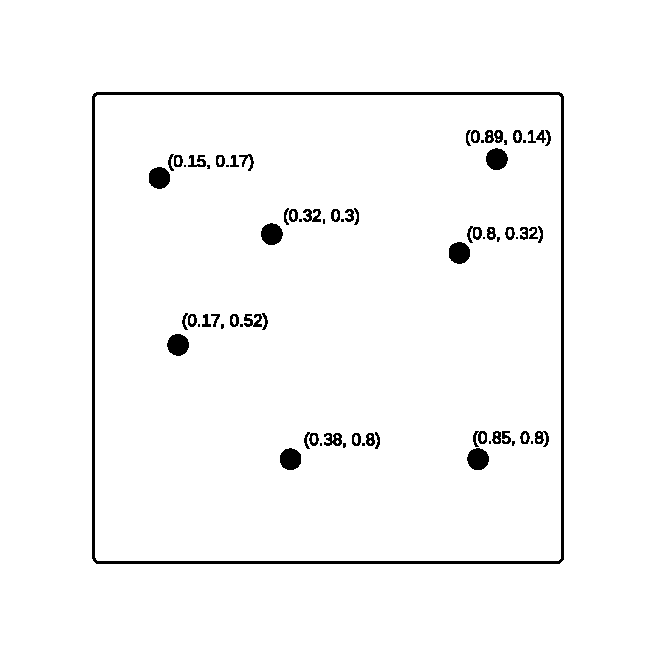
\includegraphics[scale=0.6]{figures/2D_data_space.pdf}
	\end{center}
	\vspace{-40pt}
	\caption{Data items represented as 2D points in the space $[0, 1]^d$ (not to scale)}
	\label{fig:data-space}
\end{wrapfigure}

The purpose of an index structure is to perform queries on the data. Common types of query include:
\begin{itemize}
	\item \textbf{Point Query} -- checks if a point $p$ exists in the structure \cite{rplus-tree}
	\item \textbf{Region/Range Query} -- return all points contained within a spatial region $r$ \cite{rplus-tree}, which is often a $d$-dimensional box \cite{r-tree, pk-tree, pyramid-tree}
	\item \textbf{\textit{k}-Nearest Neighbour Search} -- return the $k$ nearest points to a point $p$ \cite{pk-tree}
	\item \textbf{Approximate Nearest Neighbour Search} -- return an approximation of a $k$-nearest neighbour search \cite{knn-curse-of-dimensionality} (less accuracy, faster queries)
\end{itemize}

An index structure provides a mechanism for accessing multi-dimensional data, but it may not actually store the data itself. In a database for example, a point query comes in two parts: \textbf{searching} for a data point in the structure and \textbf{reading} the data from the data file represented by point (or index) \cite{rsr-tree}.

\section{Challenges in Multi-dimensional Search}
\label{sec:challenges}

A significant number of index structures were developed in the 1970s and 1980s, which were shown to provide good performance through empirical usage. Despite the efficiencies gained from these foundational structures, there are still numerous challenges to overcome. As such, work on developing new index structures has continued throughout the past twenty years \cite{md-structures-samet}. With the size and dimensionality of data increasing, some of these existing structures start to perform extremely poorly.

Four core challenges repeatedly discussed in the literature have been identified. Many attempts have been made to mitigate the effects of these challenges through new or modified index structures. This section will discuss these challenges, the impact they have on multi-dimensional search efficiency and \textit{why} they have these impacts.

\subsection{Curse of Dimensionality}
\label{sec:curse-of-dimensionality}

The curse of dimensionality is a term used to refer to the issues that occur when data with large numbers of dimensions is processed \cite{curse-of-dimensionality}. Spatial partitioning of high-dimensional points becomes difficult because large regions of the data space are empty. High-dimensional space is sparse because the number of data points that must be sampled to fill the space increases exponentially with $d$.

Sparsity causes many index structures to contain many empty or near-empty regions, resulting in a large amount of memory overhead (e.g. many regions in octrees with high $d$ are completely empty but exist anyway to due to uniformly sized regions). This is especially problematic when many of the dimensions might not tell you anything relevant about the data \cite{irrelevant-dimension}, causing large amounts of memory and computation to be wasted. Relating this back to multi-dimensional search specifically, Indyk and Motwani in \cite{knn-curse-of-dimensionality} discuss how efficient nearest neighbour queries with a small number of dimensions is ``well-solved", but with a high number of dimensions the problem is more challenging.

The majority of index structures discussed in the literature are hierarchical. Due to data sparseness caused by a higher number of dimensions, these structures often become very large and have many empty or near-empty nodes. Additionally, balanced splits and overlapping node regions cause most of the nodes to pass boundary intersection tests when a higher number of dimensions are used. This means the execution time of queries and dynamic operations tend to $O(n)$. In other words, the structures are no faster than a brute force sequential scan through a list, just with more memory overhead.

Weber, Schek and Blott in \cite{va-file} show how hierarchical index structures which perform data space partitioning tend to perform poorly when 10 or more dimensions is used. They even show that there is no index structure ``based on clustering or partitioning which does not degenerate to a sequential scan if the dimensionality exceeds a certain threshold" \cite{va-file}.

Therefore, for high $d$, sequential scan or methods based on linear data structures (e.g. lists) often provide better performance than methods which recursively decompose space into tree structures \cite{md-structures-samet}. This leads to the conclusion that the curse of dimensionality removes many of the benefits gained from using traditional index structures when high dimensional data is used.

\subsection{Variation in Data}

When developing an index structure, one does not know the nature of the input data in advance. Therefore, it is unwise to make too many assumptions when evaluating the efficiency of your structure with test data. Some datasets may be uniform, some may have noticeable skew and others may have a large number of clusters with complex shapes in data space. Different index structures are more efficient with different kinds of data. For example, octrees become inefficient with skewed data and $kd$-tree variants often have poor utilisation of nodes \cite{bkd-tree} (i.e. nodes store very few data points).

For some applications, where the input data's structure may be known in advance, this is not an issue, since an index structure known to perform well with that type of data can be chosen. If the nature of the data is not known in advance however, developing a generic index structure that provides efficient queries for \textit{all} kinds of data is challenging.

Wang et al. evaluated the PK-tree using uniformly distributed and clustered synthetic data, in addition to large real data sets \cite{pk-tree}. Berchtold et al. also used a combination of carefully generated synthetic data and real data sets when evaluating the performance of Pyramid Tree \cite{pyramid-tree}. Doing so allows for a comprehensive evaluation on how well a structure performs on different kinds of data.  Comprehensively evaluating an index structure's performance requires a varied collection of data, which includes:
\begin{itemize}
	\item Uniformly distributed data
	\item Non-uniform data (skewed and clustered)
	\item Large real world data sets
\end{itemize}	
Generating or finding these types of data \textit{and} ensuring an index structure performs well on most inputs have been found to be significant challenges.

\subsection{Dynamically Constructing Structures}

To maintain performance, it is common to impose invariants that maintain a balanced structure. An invariant is a condition or property of the index structure that \textit{must hold} to ensure good performance of queries. This is easier for static index structure because the structure is built once and never changes. When inserting, deleting or updating points with dynamic index structures, maintaining invariants can be non-trivial. An example of a dynamic index structure is the red-black tree, which repeatedly rotates components of the tree to fix broken invariants when a point is inserted or deleted \cite{introduction-to-algorithms}.

These invariants can result in \texttt{insert}, \texttt{update} and \texttt{delete} operations being slow. Creating index structures that provide fast queries without requiring invariants that are expensive to maintain is difficult. The balance between dynamic construction performance and query performance depends on the application. If the index structure must be updated often, then prioritising fast construction over fast queries may be appropriate.

\subsection{Memory Access and Paging}
\label{sec:paging}

Different index structures have different storage requirements. It is important to consider this when choosing/developing an index structure. Structures whose size in memory grows quickly as the amount of data increases may not be able to fit entirely in main memory, meaning some of it will have to be \textit{paged} in secondary memory (e.g. hard disk). This drastically affects performance, as it is much slower to access the hard disk than accessing main memory. This issue is amplified for high-dimensional data, as more memory is consumed per data item.

Some structures require little additional data to maintain the structure, such as splay trees and pyramid trees \cite{splay-tree, pyramid-tree}. These have \textit{low memory overhead}, meaning they scale well to large data sets. Other structures, such as PK-trees, require more data because more complex book-keeping is required to enable fast dynamic operations and queries \cite{pk-tree}. If a problem deals with massive amounts of data points, it may be worth using slower index structures with less overhead, in order to minimise the amount of memory used by the index structure. If the structure grows so large that it cannot fit in main memory, then \textit{any} index structure's performance will take a drastic hit because data has to be retrieved from secondary memory frequently.

For large datasets (terabytes in size, say), it is inevitable that some of the index structure will be stored in secondary memory. This core bottleneck has been identified and researchers have constructed index structures, called bucket methods, that store data items in ways that minimise I/O operations \cite{md-structures-samet}. Some structures have parameters that can be tweaked to find optimal paging with the target hardware or dataset, such as the PK-tree and pyramid tree \cite{pyramid-tree, pk-tree}.

To conclude, if the index structure is used with large, complex data items then some of it may have to be stored in secondary storage, especially if there are many data points. Designing an index structure to facilitate quick access to secondary memory and reduce query times has been the focus of many researchers in the field  \cite{rsr-tree, rs-tree}.

\section{Existing Index Structures}
\label{sec:structures}

Many index structures have been developed throughout the past forty years, such as quadtrees in the early 1970s \cite{quadtree} and splay quadtrees in 2012 \cite{splay-quadtree}. New structures are often based on older index structures, either by modifying an existing structure or combining two different structures in some way. Figure \ref{fig:structure-taxonomy} in Appendix \ref{chap:supp-material} shows a \textit{taxonomy} of index structures. This section describes some of the widely used index structures, their limitations (with respect to the challenges discussed in Section \ref{sec:challenges}) and why this led onto the development of new structures.

\subsection{Basic Structures}
\label{sec:basic-structures}

\textbf{Sequential scan} refers to the brute-force approach of searching a data set. You simply store the dataset in a linear data structure (e.g. a list) and iterate through each data item until the desired point is found. This means searching is an $O(n)$ operation. Using a standard array, insertion is $O(1)$ if new points are inserted at the end of the array and deletion is $O(n)$. There is little memory overhead for this approach, but search times will be very long if there are large number of points. Nevertheless, if the number of data items is small, a more complex index structure may not be needed.

\textbf{Search trees} are often used to order data items in a hierarchical fashion to make search faster \cite{introduction-to-algorithms}. The binary search tree, for one-dimensional data, is one of the first of these trees and is the basis of many index structures \cite{introduction-to-algorithms}. Each node stores a \textit{key}, which is a total orderable element. Each non-leaf node has at most two children, where the left child's key is less than its parent's and the right child's key is greater than or equal to its parent's. This property is referred to as \textit{key order} \cite{rst}. When inserting or deleting new points, the key order invariant must be maintained. Maintaining this invariant can be done in $O(n)$ time \cite{introduction-to-algorithms}, making insertion and deletion $O(n)$.

A point query is equivalent to checking if a certain key is stored in the tree. In the best case, we get running time $O(\log_2 n)$ for the query, as the height of the tree is $\log_2 n$. However, this performance is not guaranteed. Skewed or sorted data may result in taller trees, where there are many nodes with only left or only right children. This makes the binary tree \textit{unbalanced} (height greater than $\log_2 n$). If balance is not guaranteed, the running time of a point query is $O(n)$ in the worst case, which is no better than a sequential search.

\textbf{Balanced search trees} re-order the nodes to maintain balance (logarithmic height) when a node is inserted, updated or deleted, regardless of data skew. These operations cause dynamic index structure operations to become slower, but allow for faster queries. Examples of balanced search trees include red-black trees, AVL trees, splay trees and treaps \cite{introduction-to-algorithms}.

\subsection{Recursive Partitioning of Data Space}
\label{sec:recursive-partition-structures}

Index structures which decompose the data space into sub-spaces recursively are popular \cite{md-structures-samet}. The decomposed space is represented as a search tree. If $R$ is some $d$-dimensional data space, then $R_1,...,R_x$ are the decomposed sub-spaces (often disjoint) of $R$ . $R$ becomes the root node and $R_1,...,R_x$ become the children of $R$ in the tree representation. Each of those sub-spaces may then be decomposed in a similar way, increasing the depth of the tree.

This is useful because it allows large amounts of the data space to be discarded from consideration at once. Consider a point query with a point $p$. $p \in R$ since R is the entire data space. Assuming a disjoint decomposition was used, if $p \in R_1$ then $p \not\in R_2,...,R_x$. Since it is known that $p$ is only in $R_1$, only $R_1$'s children need to be checked -- the rest of the tree can be \textit{ignored}.

\subsubsection{Quadtrees}

A quadtree is one of the earliest index structures based on disjoint recursive decomposition of space, specifically created for two-dimensional space \cite{original-quadtree}. \textbf{Octrees} are a generalisation of quadtrees to $d \geq 2$ dimensions. Throughout the past forty years, many variations of the quadtree have been produced. Hanan Samet produced a survey describing many uses and variants of this data structure in  \cite{quadtree} and twenty years later, there are even more variants. Several variants are discussed in this review, but it is beyond the scope of this report to list all of them.

PR quadtrees are a commonly used quadtree which partition the data space into four uniformly sized sub-spaces. This process can be repeated recursively to produce a grid with increasingly smaller cells. Figure \ref{fig:quadtree-clustered} shows an example of a PR quadtree decomposition of some data. Notice how the underlying data space is decomposed in the same way, regardless of where the points in the dataset are in the space.

An advantage of PR quadtrees is that there is no overlap between the spatial regions represented by two sibling nodes. This greatly simplifies \texttt{insert}, \texttt{update} and \texttt{delete} operations. However, they do not perform well with \textbf{non-uniform} data. So if there are clusters or skews of data, then there will be many empty (or near empty) quadtree nodes/regions (see Figure \ref{fig:quadtree-clustered}). These unnecessary nodes in sparse regions of the data space may be searched during a query, reducing performance.

\begin{figure}
	\begin{center}
		\begin{subfloat}[PR Quadtree\label{fig:quadtree-clustered}]{%
			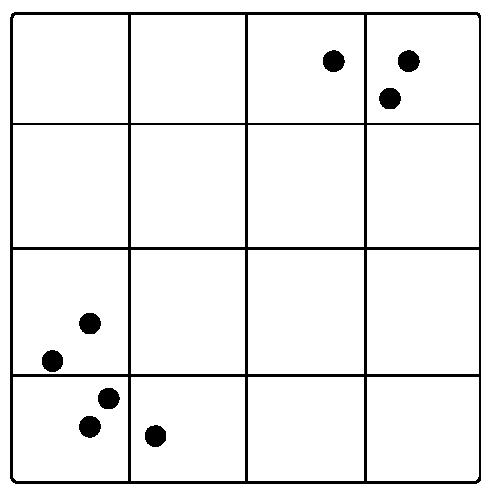
\includegraphics[scale=0.4]{figures/quadtree_clustered.pdf}
		}
		\end{subfloat}~~~~~
		\begin{subfloat}[Point $kd$-Tree\label{fig:kdtree-clustered}]{%
			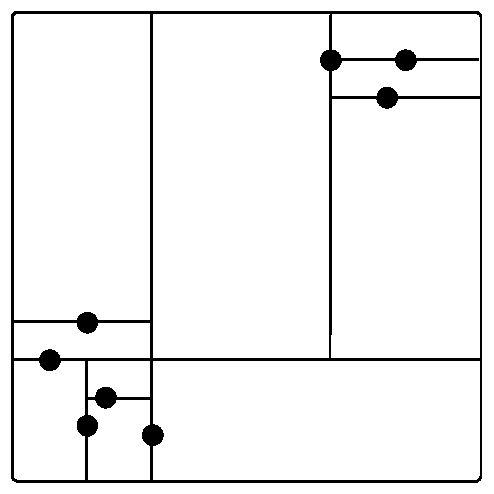
\includegraphics[scale=0.4]{figures/kdtree_clustered.pdf}
		}
		\end{subfloat}~~~~~
		\begin{subfloat}[Binary Space Partition\label{fig:bsp}]{%
			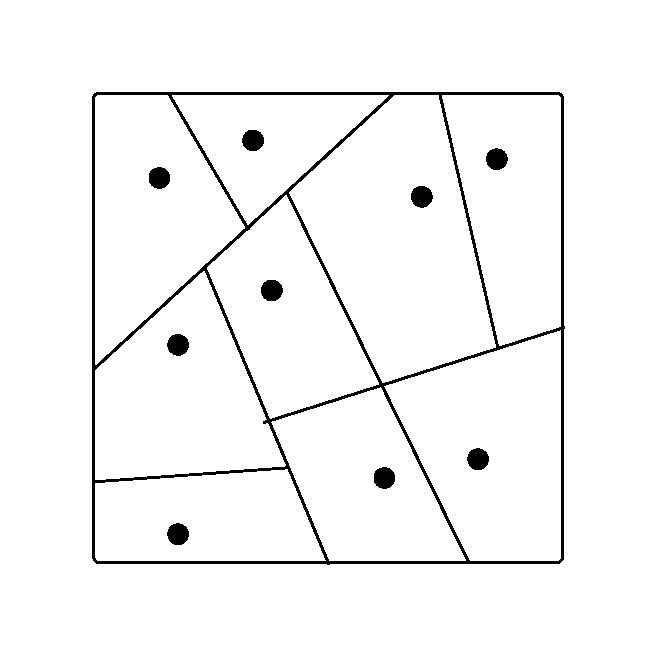
\includegraphics[scale=0.4]{figures/bsp_tree.pdf}
		}
		\end{subfloat}
	\end{center}

	\caption{Spatial Decompositions Created With Various Tree-Based Index Structures}
	\label{fig:tree-based-decomposition}
\end{figure}

\subsubsection{$kd$-trees}

$kd$-trees are similar to quadtrees in that the data space is partitioned into disjoint regions \cite{kd-tree}. Unlike quadtrees, nodes have at most two children regardless of dimensionality. Each node in the tree splits the current region of data space into two sub-regions along a single dimension $d_i$. These sub-regions are represented as two nodes, whose parent is the node representing the original region. A \textit{pivot} value $p$ is chosen for $d_i$. The left and right children contain all the data items whose $d_i$th value is less than $p$ and greater than or equal to $p$ respectively. How a $kd$-tree is built depends on how $d_i$ and $p$ are chosen, so there are many variations of this structure. There are two major types of $kd$-tree -- point and bucket (PR) \cite{md-structures-samet}. Point $kd$-trees store a single point in each node of the tree, meaning there are always $n$ nodes. Bucket $kd$-trees only store points in the leaves, which can contain multiple points.

Unlike the PR quadtree, $kd$-trees can produce non-uniform partitions, making the structure better suited to skewed or clustered data. Figures \ref{fig:quadtree-clustered} and \ref{fig:kdtree-clustered} show a PR quadtree and point $kd$-tree partition of some clustered data. Notice how there are more empty regions in the quadtree than the $kd$-tree, thus having a less efficient partition of the data.

Like binary search trees, it is ideal to maintain a \textit{balanced} tree to minimise height and ensure queries can be performed quickly. Dynamically inserting or deleting points can unbalance the tree. Variants of bucket $kd$-trees have been developed to maintain a balanced tree and fast query times. Examples of such variants include the BD-tree \cite{kdtree-v-bdtree} and KDB-tree \cite{kdb-tree}.

\subsubsection{Binary Space Partitioning}

BSP (binary space partitioning) trees are a generalisation of kd-trees that use hyperplanes (lines in 2D, planes in 3D) to recursively partition the data space \cite{bsp-tree}. That is, it partitions data space $S$ into two disjoint sub-spaces $S_1$ and $S_2$. This process is repeated recursively using different hyperplanes for each split. A BSP tree decomposition is illustrated in Figure \ref{fig:bsp}.

Optimal BSP trees allow efficient point queries to be performed by discarding as many points as possible at each level of the tree (i.e. the tree has low height). Finding optimal BSP trees for a given set of data points is an $\mathbb{NP}$-complete problem \cite{bsp-np-hard}. When inserting, updating or deleting points a new optimal partitioning must be computed to minimise tree height, making dynamic operations very slow. Therefore, BSP trees are better suited for static data because an optimal tree can be \textit{pre-computed} and loaded into main memory during program initialisation.

\subsubsection{Skip Quadtree}

Despite the original quadtree structure being developed approximately forty years ago, researchers are still enhancing the index structure's performance in new ways. A relatively new data structure, the skip quadtree, is ``simple" to implement and benefits from low memory overhead \cite{skip-quadtree}. \textbf{Skip quadtrees} were developed with range queries in mind and are based on the concept of compressed quadtrees. \textbf{Compressed quadtrees} compress paths of nodes which only have a single non-empty child into a \textit{single node} \cite{compressed-quadtree}, which combats the effects of skewed data.

Skip quadtrees combine one-dimensional skip lists \cite{skip-quadtree} and compressed quadtrees to create an index structure with $O(\log n)$ point queries and $O(\epsilon^{1 - d} \log n + k)$ \textit{approximate} range queries, where $k$ is the size of the range and $\epsilon$ is the approximation factor that controls the accuracy of the range query \cite{skip-quadtree}. However, skip quadtrees may not be efficient for very datasets because they were not constructed with paging in mind.

\subsection{Bucket Methods}
\label{sec:bucket-methods}

\textbf{Bucket methods} were developed to increase I/O efficiency for large datasets that are paged in secondary memory. Such structures were designed to minimise the number of I/O operations (secondary memory accesses) required to perform queries (see Section \ref{sec:paging}). These methods group points into contiguous memory called \textbf{buckets}, which are the same size as a page in secondary memory. To reduce the number of I/O operations required to perform a query, bucket methods aim to fill each bucket with as many nodes as possible \cite{md-structures-samet}.

There are two types of bucket methods \cite{md-structures-samet}:
\begin{itemize}
	\item \textbf{Overlapping Decomposition} -- these ensure that each bucket has a \textit{minimum} number of data items it must contain, which increases fanout and thus, search times. However, in the process of ensuring each bucket has a minimum amount of used capacity, the bounding regions of buckets in data space may begin overlapping. Overlapping regions means more nodes must be checked when performing a query, increasing search times.
	\item \textbf{Disjoint Decomposition} -- these ensure that there is \textit{no overlap} between buckets. This means less nodes need to be checked in a query, but there is no guarantee on how much each bucket is filled, potentially increasing the number of I/O operations performed
\end{itemize}

\textbf{Fanout} refers to the amount of children each node have on average. Higher fanout results in a search tree with lower height, which means less nodes are accessed on average when searching for a point. Node access is particularly expensive when the tree has been paged into secondary memory, so some bucket methods aim to increase fanout (e.g. TV-tree \cite{tv-tree} and A-tree \cite{a-tree}).

\subsubsection{B-Trees and B${}^{+}$-Trees}

The B-Tree was developed by Rudolf Bayer in 1972 and is often used for databases or file-systems \cite{ubiquitous-btree}. It is a one-dimensional search tree which allows for point queries, insertions and deletions to be performed in $O(\log n)$ time \cite{btree}. B-trees maintain key order, but allow nodes to have more than two children, making them a generalisation of binary search trees.

B${}^{+}$-trees are B-trees where only the \textit{leaves} contain the actual values of the data \cite{ubiquitous-btree}. This means all non-leaves simply contain pointers to, or the keys of, their children. B${}^{+}$-trees ensure that each bucket is at least 50\% full \cite{md-structures-samet, ubiquitous-btree}, which leads to less I/O operations. This is a very attractive property, as it can greatly speed up query times for large data sets. There have been many attempts to generalise the B-tree to a multi-dimensional setting while retaining this property. The k-d-B tree \cite{kdb-tree} and BV-tree \cite{bv-tree} are two examples of such attempts. Freeston in \cite{bv-tree} discusses how this ``apparently simple" objective has proved extremely difficult to achieve.

\subsubsection{R-Tree Family}

An R-tree can be thought of as a B${}^{+}$-tree that can handle multi-dimensional data, supporting data items that have non-zero size in data space (i.e. regions) \cite{r-tree}. This means nodes are represented using \textit{hyper-rectangles} that define the region of the data space all of the node's children are contained in. The running time for queries is $O(n)$ in the worst case, but expected performance is much higher. There are many variations of R-trees that have improved performance, such as R*-trees \cite{rstar-tree}, R+-trees \cite{rplus-tree}, SS-trees \cite{ss-tree}, RS-trees \cite{rs-tree} and Hilbert R-Trees \cite{hilbert-rtree}. Combinations of these variations also exist, such as SR-trees \cite{md-structures-samet} and RSR-trees \cite{rsr-tree}.

R-tree based structures use overlapping decomposition, which is a key performance issue \cite{pyramid-tree}. If you have a point contained in $m$ nodes' regions, all $m$ nodes could be searched. This severely limits the performance of R-tree based index structures with data spaces that have a \textbf{large} number of dimensions (see Section \ref{sec:curse-of-dimensionality} for more details).

\subsubsection{PK-Tree}

PK-trees (Pyramid K-instantiable trees) are a family of structures based on kd-trees that were created specifically to handle high-dimensional data \cite{pk-tree}. They are similar to bucket methods, but instead of imposing a minimum number of points per bucket, they impose a maximum. Imposing this maximum (called the $k$-instantiation value) results in a reduced amount of I/O operations \cite{md-structures-samet}. PK-trees bound the height of the tree to $O(\log n)$ for some data. Through tests on synthetic and real data, the PK-tree has been shown in greatly outperform the SR-tree and X-tree \cite{pk-tree}, especially for higher dimensions.

However, there are some caveats. In order for the PK-tree to have $O(\log n)$ height, certain constraints must be applied to the distribution of the data. Furthermore, the pagination of the index structure which minimises I/O operations depends on the value of $K$ (the number of children a node can have) and the size of the actual hard disk pages used by the operating system \cite{pk-tree}. The amount to split each dimension at each level is also configurable, so there are many parameters to tweak to achieve the proposed performance. Additionally, as discussed in Section \ref{sec:curse-of-dimensionality}, the PK tree's performance on very high dimensional data will be still be poor, because most index structures that decompose the underlying data space perform poorly when $d$ is high.

PK-trees are also complicated to implement. This problem is exacerbated by having to tweak many different parameters and be careful about what kind of data is stored in the tree. Therefore, due to their complexity and poor performance on very high dimensional spaces, PK-trees have not been widely adopted \cite{md-structures-samet}.

\subsection{Structures Tailored to High-Dimensional Data}
\label{sec:high-dimensional-structures}

Section \ref{sec:curse-of-dimensionality} discusses how higher dimensional data spaces cause index structures which perform well on low dimensional data to degenerate and provide poor performance. There have been efforts to develop index structures which still perform well in these data spaces. Many different approaches have been used, such as tree-based spatial decompositions, distance-based methods, dimension reduction and non-hierarchical, sequential methods. Some of the more influential data structures from the literature have been identified and are described here.

\subsubsection{X-Tree}

R-tree based index structures often struggle to provide efficient queries in high-dimensional space, because the hyper-rectangles or spheres tend to overlap more \cite{pyramid-tree}. X-trees \cite{x-tree} try to reduce overlap by extending the capacity of nodes/buckets if creating a new node would result in an overlap (these are called supernodes). X-trees outperform most R-tree variants \cite{x-tree}. However, Berchtold et al. show in  \cite{pyramid-tree} show the structure still degenerates at higher dimensions ($d \geq 10$) \cite{pyramid-tree}.

\subsubsection{Distance-Based Methods}

When there are a large number of dimensions, determining which dimensions are actually relevant for searching can be difficult. In these cases, \textbf{distance-based methods} may be useful. They use the similarity (distance in data space) between each pair of points to deduce more information about the relationships in the data and provide faster search \cite{md-structures-samet}. There are two major types: \textbf{pivot-based}, which choose a subset of all points in the dataset to base distance measurements on, and \textbf{cluster-based}, which partition the dataset's points into spatial regions called clusters that are used to compute distances \cite{md-structures-samet}. A notable distance-based index structure is the M-tree, which combines R-trees with distance-based techniques to perform high dimensional search with dynamic datasets \cite{m-tree}.

\subsubsection{Dimension Reduction}

One method of mitigating the effects of the curse of dimensionality is reducing the dimensionality of the dataset and then using an existing structure which is known to have good performance with low dimensional data. One example of this is principal component analysis (PCA) \cite{pca}, which transforms a data space into one with less dimensions, using correlations in the data to deduce with dimensions are the most useful for discrimination \cite{pca}. However, by reducing the dimensions using PCA some information is lost and the results of queries will not be exact. Note that PCA is an equivalent technique to SVD (Singular Value Decomposition) \cite{md-structures-samet}.

PCA struggles with dynamic data; if the data changes then the computed transformation will go out of sync and queries will be even less accurate. The transformation could be re-computed whenever a point is added, removed or changed but doing so takes a very long time, making dynamic operations really slow. Therefore, these dimension reducing techniques are suitable to static datasets where full accuracy is not required.

\subsubsection{Pyramid Tree}
\label{sec:pyramid-tree}

The pyramid tree is specifically targeted towards high-dimensional data \cite{pyramid-tree}. It partitions the data space into $2d$ pyramids and map $d$-dimensional data items to \textbf{one-dimensional space}, storing the mapped 1D points in a B${}^{+}$-tree. This one-dimensional representation is achieved by describing a data point in terms of \textit{which} pyramid it is contained in and \textit{where} in the specified pyramid it is. Queries are given as $d$-dimensional points which are reduced to one dimension before they're applied, reducing the effects of the curse of dimensionality. Even though data points are stored in a one-dimensional B${}^{+}$-tree, the original data is maintained since the original $d$-dimensional point is stored alongside its 1D representation. Hence, pyramid trees reduce the dimensionality of the data but retain all of the original information, unlike PCA.

B${}^{+}$-trees provide efficient \texttt{insert}, \texttt{update} and \texttt{delete} operations \cite{ubiquitous-btree}, meaning the corresponding operations are also efficient with pyramid trees. The pyramid tree's range query performance, \textit{relative} to other index structures such as X-trees, increases as $d$ does \cite{pyramid-tree}. This structure has low memory overhead because, in addition to B${}^{+}$-tree overhead, one extra value is stored per point.

Since the pyramid tree mitigates the curse of dimensionality, provides dynamic operations, uses a bucket method to store the 1D points and handles skewed data (using the Extended Pyramid Technique \cite{pyramid-tree}), the structure considers all four challenges discussed in Section \ref{sec:challenges}. Tests performed by Berchtold et al. show that the Pyramid Tree is successful at tackling these challenges \cite{pyramid-tree}.

\subsubsection{Embedding Methods}

Embedding methods are combinations of dimension reduction and distance-based methods \cite{md-structures-samet}. They use \textit{approximated} distances between points in reduced space to perform \textit{exact} queries. An example of an embedding method is FastMap \cite{fast-map}.

\subsubsection{Non-Hierarchical Methods}

Focus is turning towards sequential scan and linear data structures for faster search with high-dimensional data \cite{md-structures-samet, va-file}. This is because hierarchical index structures based on data space partitioning perform poorly on a higher number of dimensions (see Section \ref{sec:curse-of-dimensionality}). Furthermore, for large datasets that must be stored in secondary memory, sequential scan may also outperform hierarchical methods, because data items are stored contiguously and read sequentially, thus requiring less I/O operations. The VA-file is a method based on sequential scan, which is shown to consistently outperform sequential scan and the X-tree as the number of dimensions increase on real datasets \cite{va-file}.

Another non-hierarchical index structure that has been used are hash maps \cite{md-structures-samet}. One approach is to define one primary bucket in the hash map for each grid cell (region of data space), which can hold $x$ points. If a primary bucket has more than $x$ points, then an overflow bucket is constructed. This bucket is linked to the primary bucket it spawned from, similar to the chaining conflict resolution mechanism for 1D hash tables \cite{introduction-to-algorithms}. Notable hashing techniques for multi-dimensional search include MDEH (multi-dimensional extended hashing) and PLOP (piecewise linear order preserving) hashing \cite{md-structures-samet}.


\subsection{History-sensitive Structures}
\label{sec:history-sensitive-structures}

Given the same data twice, most structures will behave exactly the same. That is, how the structure builds itself and access times have little, if any, variation. There are some structures which are \textbf{history-sensitive}, meaning that their behaviour is either non-deterministic, involving some element of randomness that affects how the structure performs over time, or self-adjusting, changing itself based on how the stored data is accessed. These can allow structures to be much more dynamic and adjust themselves to perform optimal search based on the application it is being used in. Two of these structures, the quadtreap and splay quadtree, are described here.

\subsubsection{Quadtreap}

A treap is a randomised search tree used to store one-dimensional keys, which combines a binary search tree with a heap by maintaining both \textit{key-order} and \textit{heap-order} (nodes ordered by the randomly assigned probabilities) \cite{quadtreap}. The main advantage of the quadtreap is that $\log n$ height can be maintained, even when dynamically inserting and removing points, with ``high probability" \cite{quadtreap}.

A quadtreap is a combination of a compressed quadtree and a treap. Tree rotations are used to maintain a balanced height when the tree is modified. Let $h$ be the height of the tree. Running times for \texttt{insert} and point queries are $O(h)$, and \texttt{delete} is performed in $O(h^2)$. This means the \textit{expected} times for \texttt{insert} and \texttt{delete} are $O(\log n)$ and $O(\log^2 n)$ respectively.

\subsubsection{Splay Quadtree}
\label{sec:splay-quadtree}

Splay trees are one-dimensional index structures which make use of a splaying operation to achieve fast dynamic operations \cite{introduction-to-algorithms}. A splay tree is \textit{self-adjusting}, which means it is ``a data structure that reorganises itself to fit the pattern of access." \cite{splay-quadtree} This is achieved with the splaying operation, which performs a series of $O(1)$ tree rotations to maintain a balanced tree with low height.

Park and Mount, the creators of the quadtreap \cite{quadtreap}, stated ``there is no comparable self-adjusting data structure for storing multi-dimensional point sets" with regard to splay trees \cite{splay-quadtree}. Hence, they developed the splay quadtree, which combines BBD-trees (balanced box decomposition trees) with quadtrees by making use of an equivalent splaying operation on BBD-trees. Park and Mount proved good bounds on the running time of dynamic operations and queries.

The structure is complicated to implement and no papers evaluating its performance empirically have been published. Currently, the splay quadtree remains a purely theoretical structure.
\section{Evaluating and Choosing an Index Structure}
\label{sec:comparison}

\subsection{Measuring Efficiency}
\label{sec:measuring-efficiency}

One can measure the efficiency of an index structure by simply measuring the amount of time it takes perform dynamic operations and queries \cite{dynamic-data-structures}. In addition to execution time, one must also consider how much memory overhead is produced by the index structure. Such overhead may not be an issue for small data sets, but when your index structure becomes very large, it must be considered due to the issues discussed in Section \ref{sec:paging}. Measurements of index structure efficiency include:
\begin{itemize}
	\item \textbf{Structure Size} -- memory required to store the structure, relative to dataset size
	\item \textbf{Construction Time} -- how long it takes to construct a structure storing $n$ points
	\item \textbf{Dynamic Operation Execution Time} -- execution times of \texttt{insert} and \texttt{delete} operations
	\item \textbf{Query Execution Time} -- execution times of point, range or nearest neighbour queries
\end{itemize}
Big-Oh notation \cite{design-analysis-algorithms} refers to the worse case execution time of an algorithm, often with respect to the size of the input. This is used to bound the worst, average or expected execution time of an algorithm. This can be used to construct theoretical performance measurements for an index structure and if often used to guide the development and evaluation of index structures structures (e.g. in  \cite{splay-quadtree}).

The focus of bucket methods is to minimise I/O operations while still retaining well-balanced search trees. Therefore, in addition to the runtime of each operation, the number of I/O operations, or \textbf{page accesses}, is often measured (e.g. \cite{pk-tree, pyramid-tree, x-tree}). In conjunction with CPU processing time, page access count can give good insight into how efficient an index structure is for large datasets.

\subsection{Deciding on an Index Structure}
\label{sec:structure-decision}

While some structures are generally less efficient than others, such as the R-tree when compared to X-tree, the behaviour of index structures typically depends on the input data. In other words, there is no ``best" structure. Choosing the best index structure is \textit{task-dependent}. There are many factors to consider when choosing an index structure, some of which are listed below.
\begin{itemize}
	\item how many points will the structure contain?
	\item how many dimensions does the data have?
	\item how frequently will the data be modified, if at all?
	\item do queries have to be performed near real-time or is it acceptable to wait a few minutes?
	\item what distributions will the input data have? will they be uniform or highly skewed?
\end{itemize}

Note that this is by no means an exhaustive list. Table \ref{tab:comparison} in Appendix \ref{chap:supp-material} lists some of the index structures discussed in this review and their strengths and weaknesses.

The strengths and weaknesses of the structures discussed in the review will now be summarised. B${}^{+}$-trees are very popular for one-dimensional data because they are fast, simple and have low memory overhead \cite{ubiquitous-btree}. Quadtrees, kd-trees and R-tree variants have good performance on multi-dimensional data (e.g. for geometric optimisation of a 3D scene \cite{kd-tree-gpu}) and are simple to implement (no complex invariants to maintain). However, performance starts to decrease as you increase the number of dimensions. There is a need for structures which can perform efficient queries in high-dimensional space, so structures such as the pyramid tree and PK-tree were developed \cite{pk-tree, pyramid-tree}. For even higher dimensions (e.g. $d \geq 10$), it has been shown that non-hierarchical methods, such has hash-based structures or sequential scan variants, may provide better performance.
\section{Parallel Search}

When it is desired to increase the efficiency of some computational task, it is common to consider parallelisation. In the context of multi-dimensional search, this means we want to determine whether or not it's possible to perform the dynamic operations and queries of an index structure in parallel, so that we reduce runtime by solving multiple parts of the problem at once.

\textbf{Multi-core parallelisation} runs tasks in parallel on different CPU cores, which can be achieved by executing a program on multiple processes or threads on the host operating system. While it is possible to parallelise index structures on multi-core processors, prior research appears to focus on many-core (see  \cite{btree-gpu1, btree-gpu2, btree-gpu3, traversing-spatial-indexes-gpu, rtree-gpu1, rtree-gpu2}) and distributed (see \cite{fat-btree, distributed-kd-tree, distributed-md-search}) parallelisation. \textbf{Many-core} parallelisation involve a much larger number of cores than multi-core processors and thus, higher parallelisation. GPUs (graphics processing units) are examples of many-core processors, which can have thousands of cores. Despite GPUs initially being created for real-time graphics, they are increasingly being used for general-purpose computing (GPGPU) \cite{performance-tuning-gpgpu}. \textbf{Distributed computing} achieves parallelisation by having multiple physical machines performing the work, communicating with each other over a network \cite{distributed-systems}.

\textbf{Embarrassingly parallel} is a term used to describe problems which can be easily split up into independent tasks that can be parallelised \cite{designing-parallel-programs}. Queries using sequential scan can be considered embarrassingly parallel, as the linear structure can be partitioned and allocated to multiple processors which each search their own sub-structure \cite{gpu-gems-3}. Many index structures are non-linear, hierarchical structures that use some form of tree. This can make them difficult to parallelise, especially if queries require backtracking (traversing back \textit{up} the tree to take another path). This makes the parallelisation of many search structures incredibly difficult and for some, the level of communication that would be required between each parallel process is so high it dominates the time savings achieved by parallelisation, making it less efficient than a serial implementation.

A good amount of research has been performed on parallelising one-dimensional search structures, especially the B-tree, \cite{btree-gpu1, btree-gpu2, btree-gpu3, fat-btree, multidisk-btree, parallel-btree}. There has also been research into parallel multi-dimensional structures, such as the KDB-tree \cite{traversing-spatial-indexes-gpu} and R-trees \cite{master-client-rtree, parallel-rtree, rtree-gpu1, rtree-gpu2}. Recent years have seen much focus on running search on the GPU. Both the B-tree and R-tree have been successfully parallelised on the GPU and have achieved increased performance \cite{btree-gpu2, rtree-gpu1}. However, these techniques are complex and difficult to implement. It appears that parallelising multi-dimensional, even for small gains in efficiency, requires significant effort.

Furthermore, most of the multi-dimensional index structures which have currently been parallelised in the literature (e.g. R-tree) are known to degenerate when given high dimensional data (see Section \ref{sec:curse-of-dimensionality}). Since this project's focus is high-dimensional data and many of the existing parallel techniques are difficult to implement, especially for a developer with little experience with parallel or GPGPU programming, it has been decided that parallelisation will not be the focus of the project initially. For the first iteration, a serial index structure will be implemented. Depending on future research findings, later iterations may implement parallel index structures (either multi-core or many-core), but for the moment this is not the case.

\subsection{Conclusion}

In this review, the multi-dimensional search problem has been defined. Problems from many different areas of computer science, such as database querying, computer vision and visualisation, benefit from multi-dimensional search, meaning there is much benefit to gain from accelerating this process. A large array of index structures have been developed throughout the past forty years to solve this problem. Sequential scan was deemed an inefficient, na\"{i}ve solution to the problem and more sophisticated index structures were developed.

Each index structure has its own advantages and disadvantages because they were developed to tackle specific challenges. While some structures generally outperform others, there is often no ``best" structure. When considering which to use for a given application, it is important consider some key aspects about the data and the application it is being used in (see Section \ref{sec:structure-decision}). The answers to these questions can help guide the decision on which index structure to use.

The one-dimensional search problem is generally well solved and fast, dynamic index structures capable of storing huge amounts of data exist. For a low number of dimensions (e.g. 2 or 3), research has focused more on developing simple index structures with lightweight memory requirements. For high-dimensional data, focus appears to be shifting away from tree-based structures that recursively decompose space and towards linear structures. This is because tree-based approaches have been shown to have limited, if no, performance gain over sequential-based approaches when dealing with large numbers of dimensions \cite{md-structures-samet}. There has been research into parallising search, but it appears to remain a difficult problem, with little focus being given to parallelising high-dimensional search.

\chapter{Final Evaluation}
\label{chap:evaluation}
\centerline{\rule{149mm}{.02in}}
\vspace{2cm}

We have shown that the point $kd$-tree greatly outperforms the Pyramid tree for the two scientific datasets. For all synthetic data and the 3D point cloud dataset, the Pyramid tree is faster, especially with regard to point deletion.

This section will explore the reasons for this, determining which characteristics in the data cause the performance of the structures to degenerate. The section will conclude by discussing the types of data suitable for the Pyramid Tree and $kd$-Tree, along with some further discussion on the implications of the results from this evaluation.

TODO: summary of findings so far

\section{Characteristics of Test Data}

TODO


\section{Distribution of Points Across Buckets}

TODO

\section{Suitable Data for Index Structures}

TODO
\section{Next Steps: Design and Implementation}
\label{sec:next-steps}

After the submission of this report, the first iteration of the ``Design and Implementation" phase will begin. In these two weeks, the development environment will be set up and an \textbf{evaluation framework} will be created. This framework will be a C++ program that will facilate fast evaluation by allowing multiple index structures to be tested at once (using the test process described in Section \ref{sec:evaluation}), with multiple datasets. The framework will automatically generate the evaluation measures as text files and figures, so they can easily be understand and incorporated into the report. More details on the design and features of this framework will be given in the final report.

The first iteration will also implement the evaluation baselines (sequential scan and quadtree) and a chosen index structure. Initially, the Pyramid tree was going to be implemented because the structure appears to perform very well in a high-dimensional setting (based on the literature). However, through the Visualization Toolkit (VTK)\cite{vtk}, the School already has a working implementation of the Pyramid tree. Taking the School's interests into account, it was felt that implementing the Pyramid tree again, even if the new implementation has greater performance, would not provide as much insight into high-dimensional search as implementing a structure that the School does not currently have an implementation of.

Therefore, the \textbf{splay quadtree} has been chosen as the index structure to implement. It was chosen because of its self-adjusting behaviour. From the review of literature performed, it appears self-adjusting structures have not been evaluated against high-dimensional data. By implementing the splay quadtree, insight into how these types of structures perform with higher dimensions can be gained. Furthermore, the structure has low memory overhead, making it useful for storing the large astrophysics dataset described in Section \ref{sec:evaluation} whilst keeping it in main memory (see assumption (2) in Section \ref{sec:core-assumptions}). After this iteration, the remaining iterations will attempt to optimise the splay quadtree or choose to explore a different index structure if it is shown that, algorithmically, the structure performs poorly with high-dimensional data.

Additionally, the ``Final Report Write-up"" phase will begin and run in parallel with the ``Design and Implementation" phase after the first iteration.


% Include the bibliography
\bibliographystyle{unsrt}
\bibliography{refs}
\appendix
\setcounter{figure}{0} \renewcommand{\thefigure}{A.\arabic{figure}} 
\setcounter{table}{0} \renewcommand{\thetable}{A.\arabic{table}} 
\section{How Ethical Issues are Addressed}

There are no ethical issues involved with this project, as no personal data is being used in either the design, implementation or evaluation of the solution. All data used for evaluation is either synthetic data generated specifically for this project or publicly available datasets.

\section{Supplementary Material}

\begin{figure}[H]
	\centering
	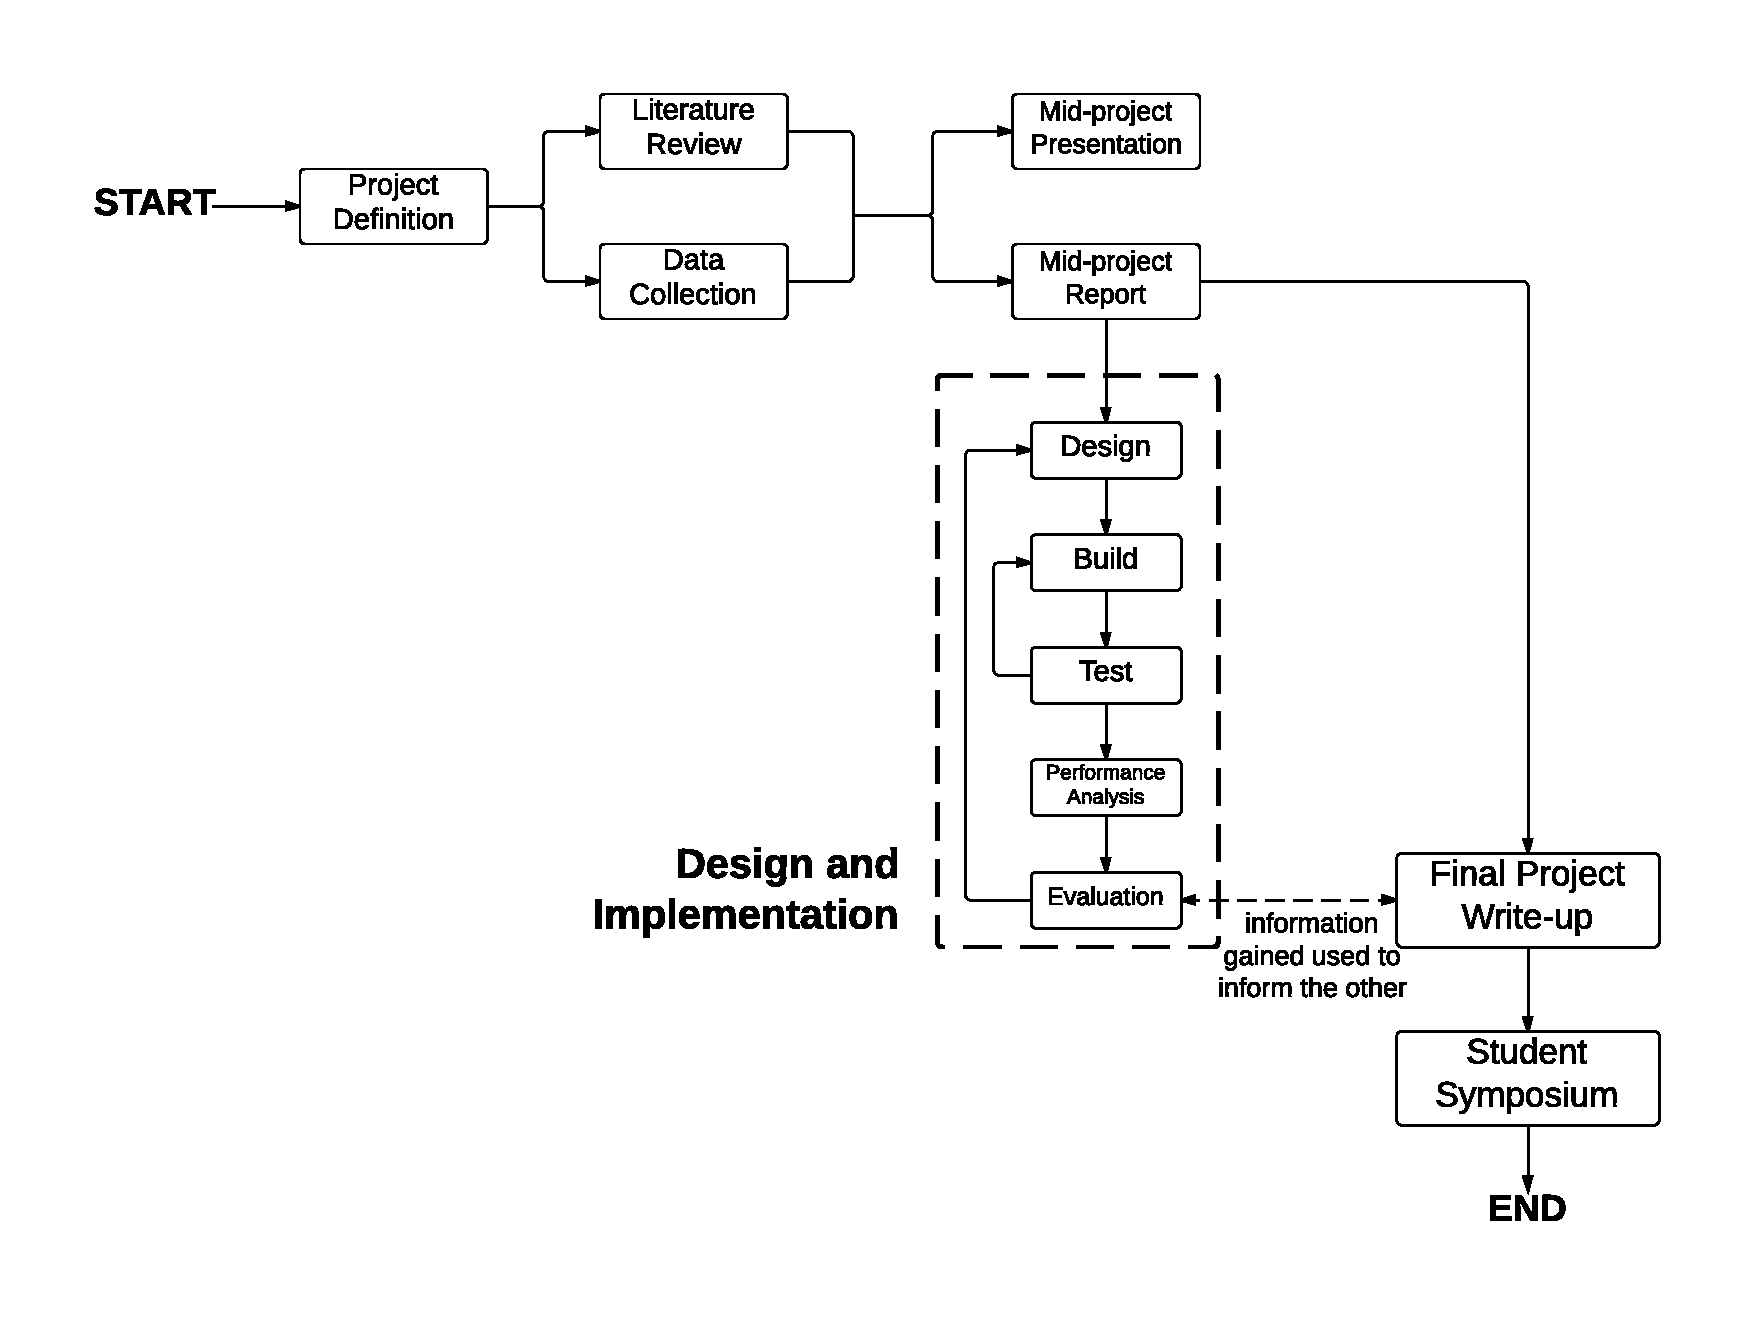
\includegraphics[scale=0.6]{figures/full-project-process.pdf}
	\caption{Flow Chart of Full Project Schedule}
	\label{fig:full-project-process}
\end{figure}

\newpage

\null  % Empty line
\nointerlineskip  % No skip for prev line
\vfill
\let\snewpage \newpage
\let\newpage \relax

\begin{figure}[H]
	\centering
	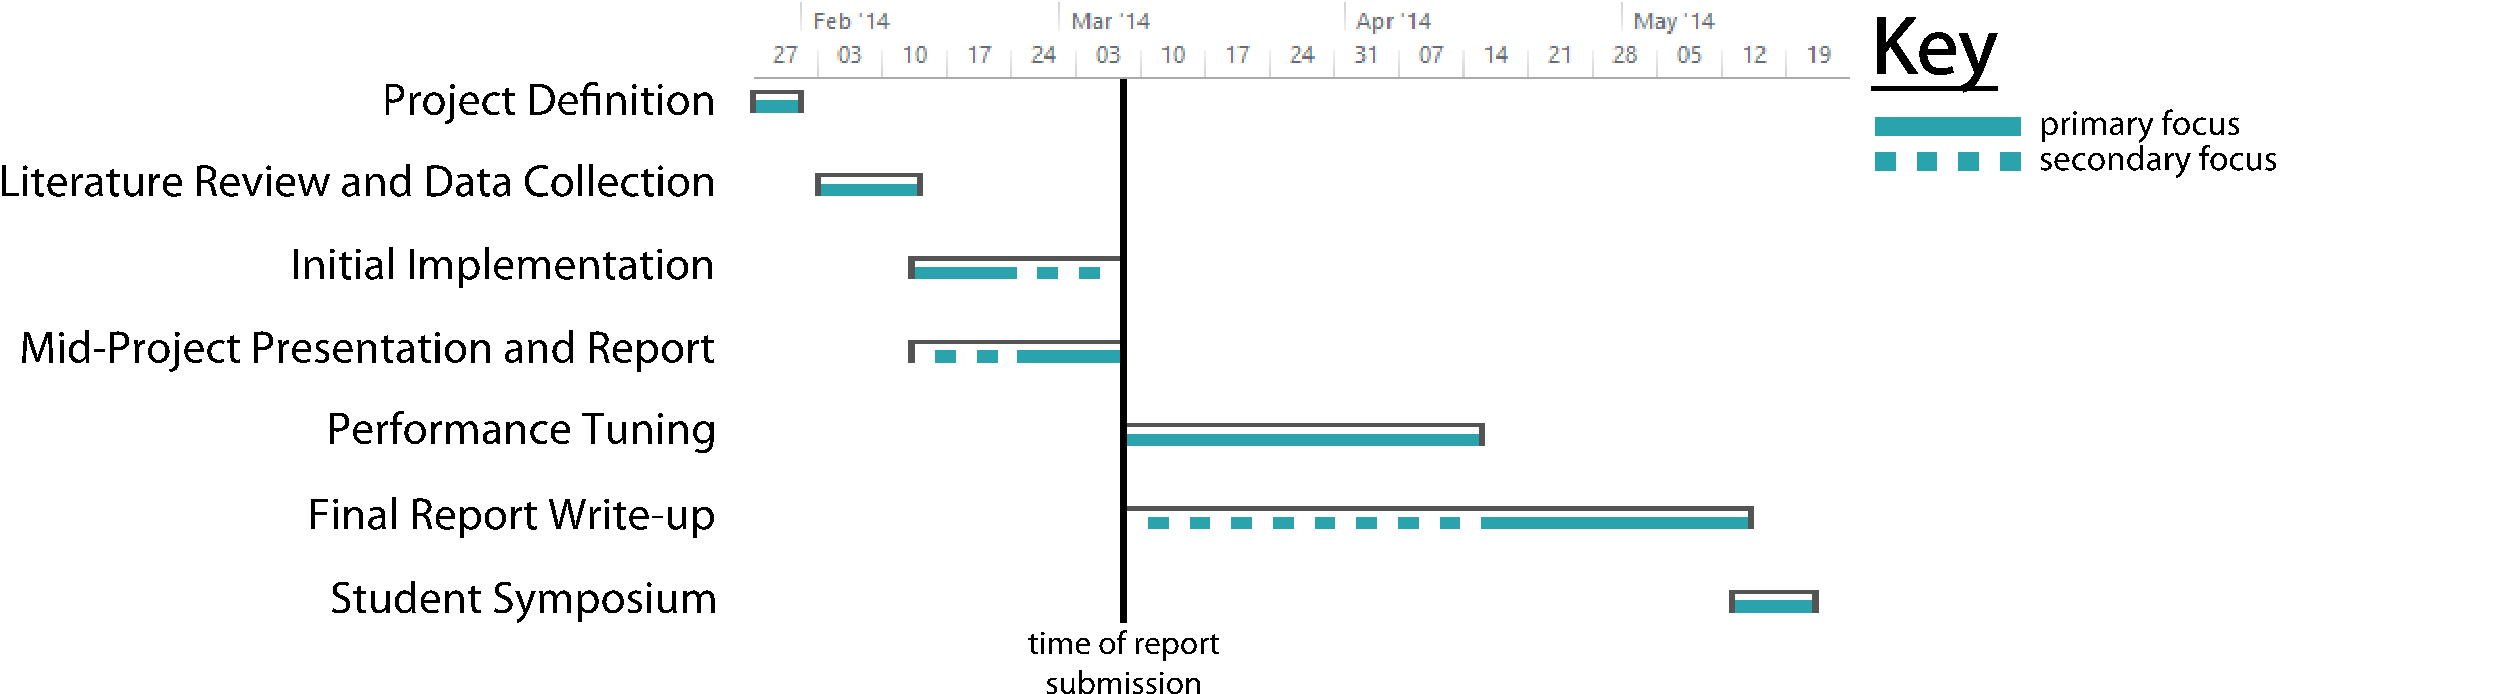
\includegraphics[scale=0.475]{figures/initial_project_schedule.pdf}
	\caption{Initial Project Schedule Created on 31/01/14. The time this report was submitted is marked on the chart to illustrate the project's current progress.}
	\label{fig:initial-schedule}
\end{figure}

\begin{figure}[H]
	\centering
	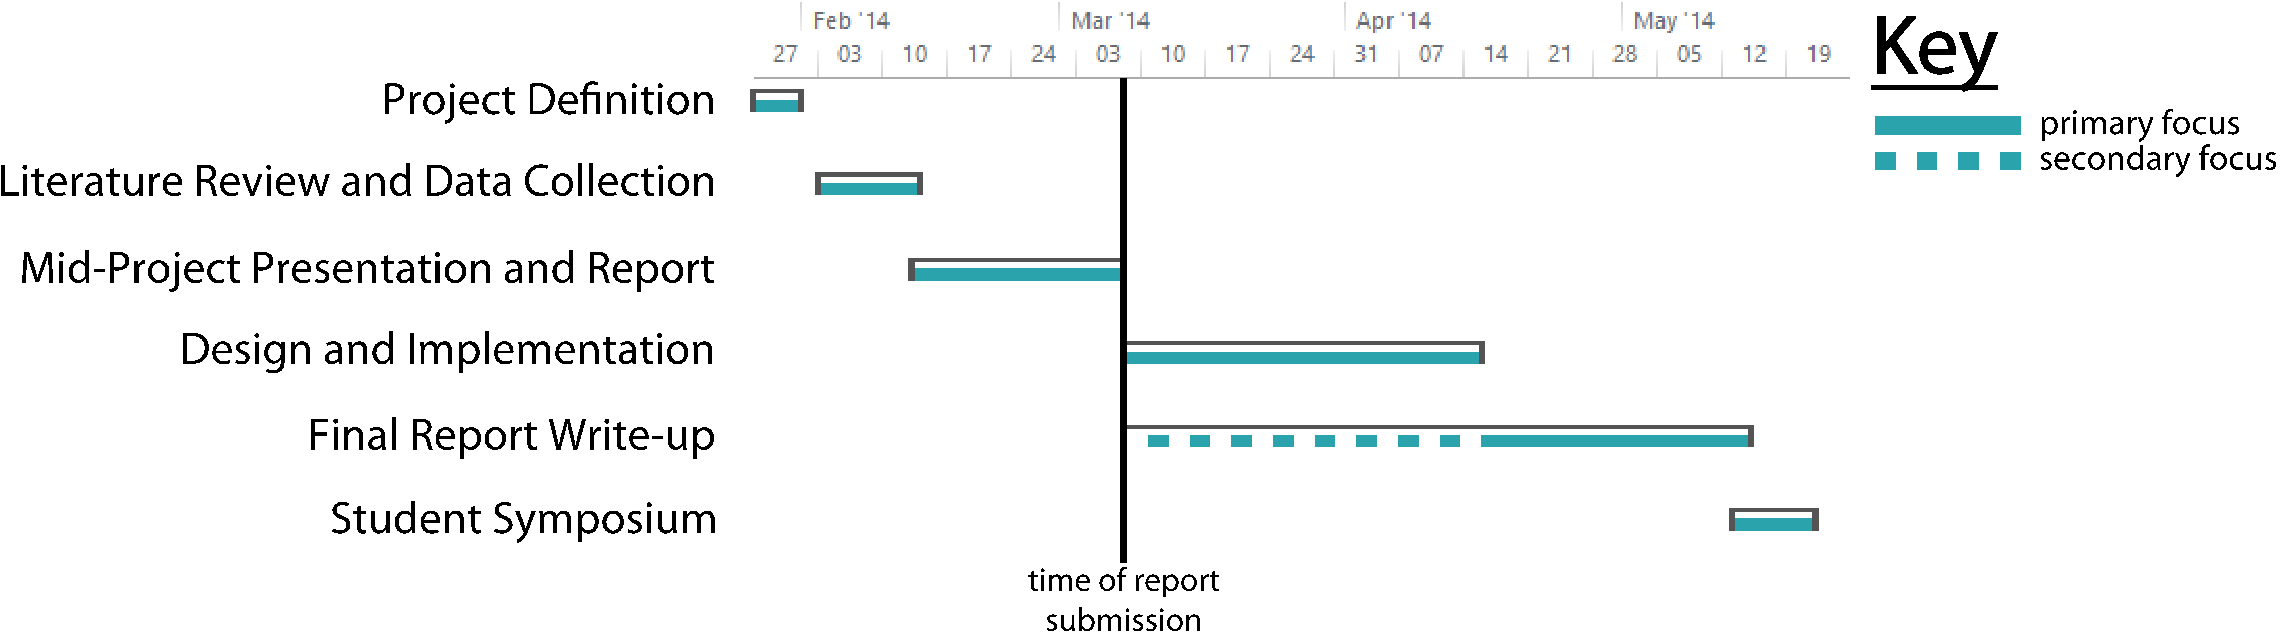
\includegraphics[scale=0.475]{figures/revised_project_schedule.pdf}
	\caption{Revised Project Schedule Created on 20/02/14. The time this report was submitted is marked on the chart to illustrate the project's current progress.}
	\label{fig:revised-schedule}
\end{figure}

\let \newpage \snewpage
\vfill 
\break % page break

\begin{landscape}	

\null  % Empty line
\nointerlineskip  % No skip for prev line
\vfill
\let\snewpage \newpage
\let\newpage \relax
	\begin{figure}[H]
		\centering
		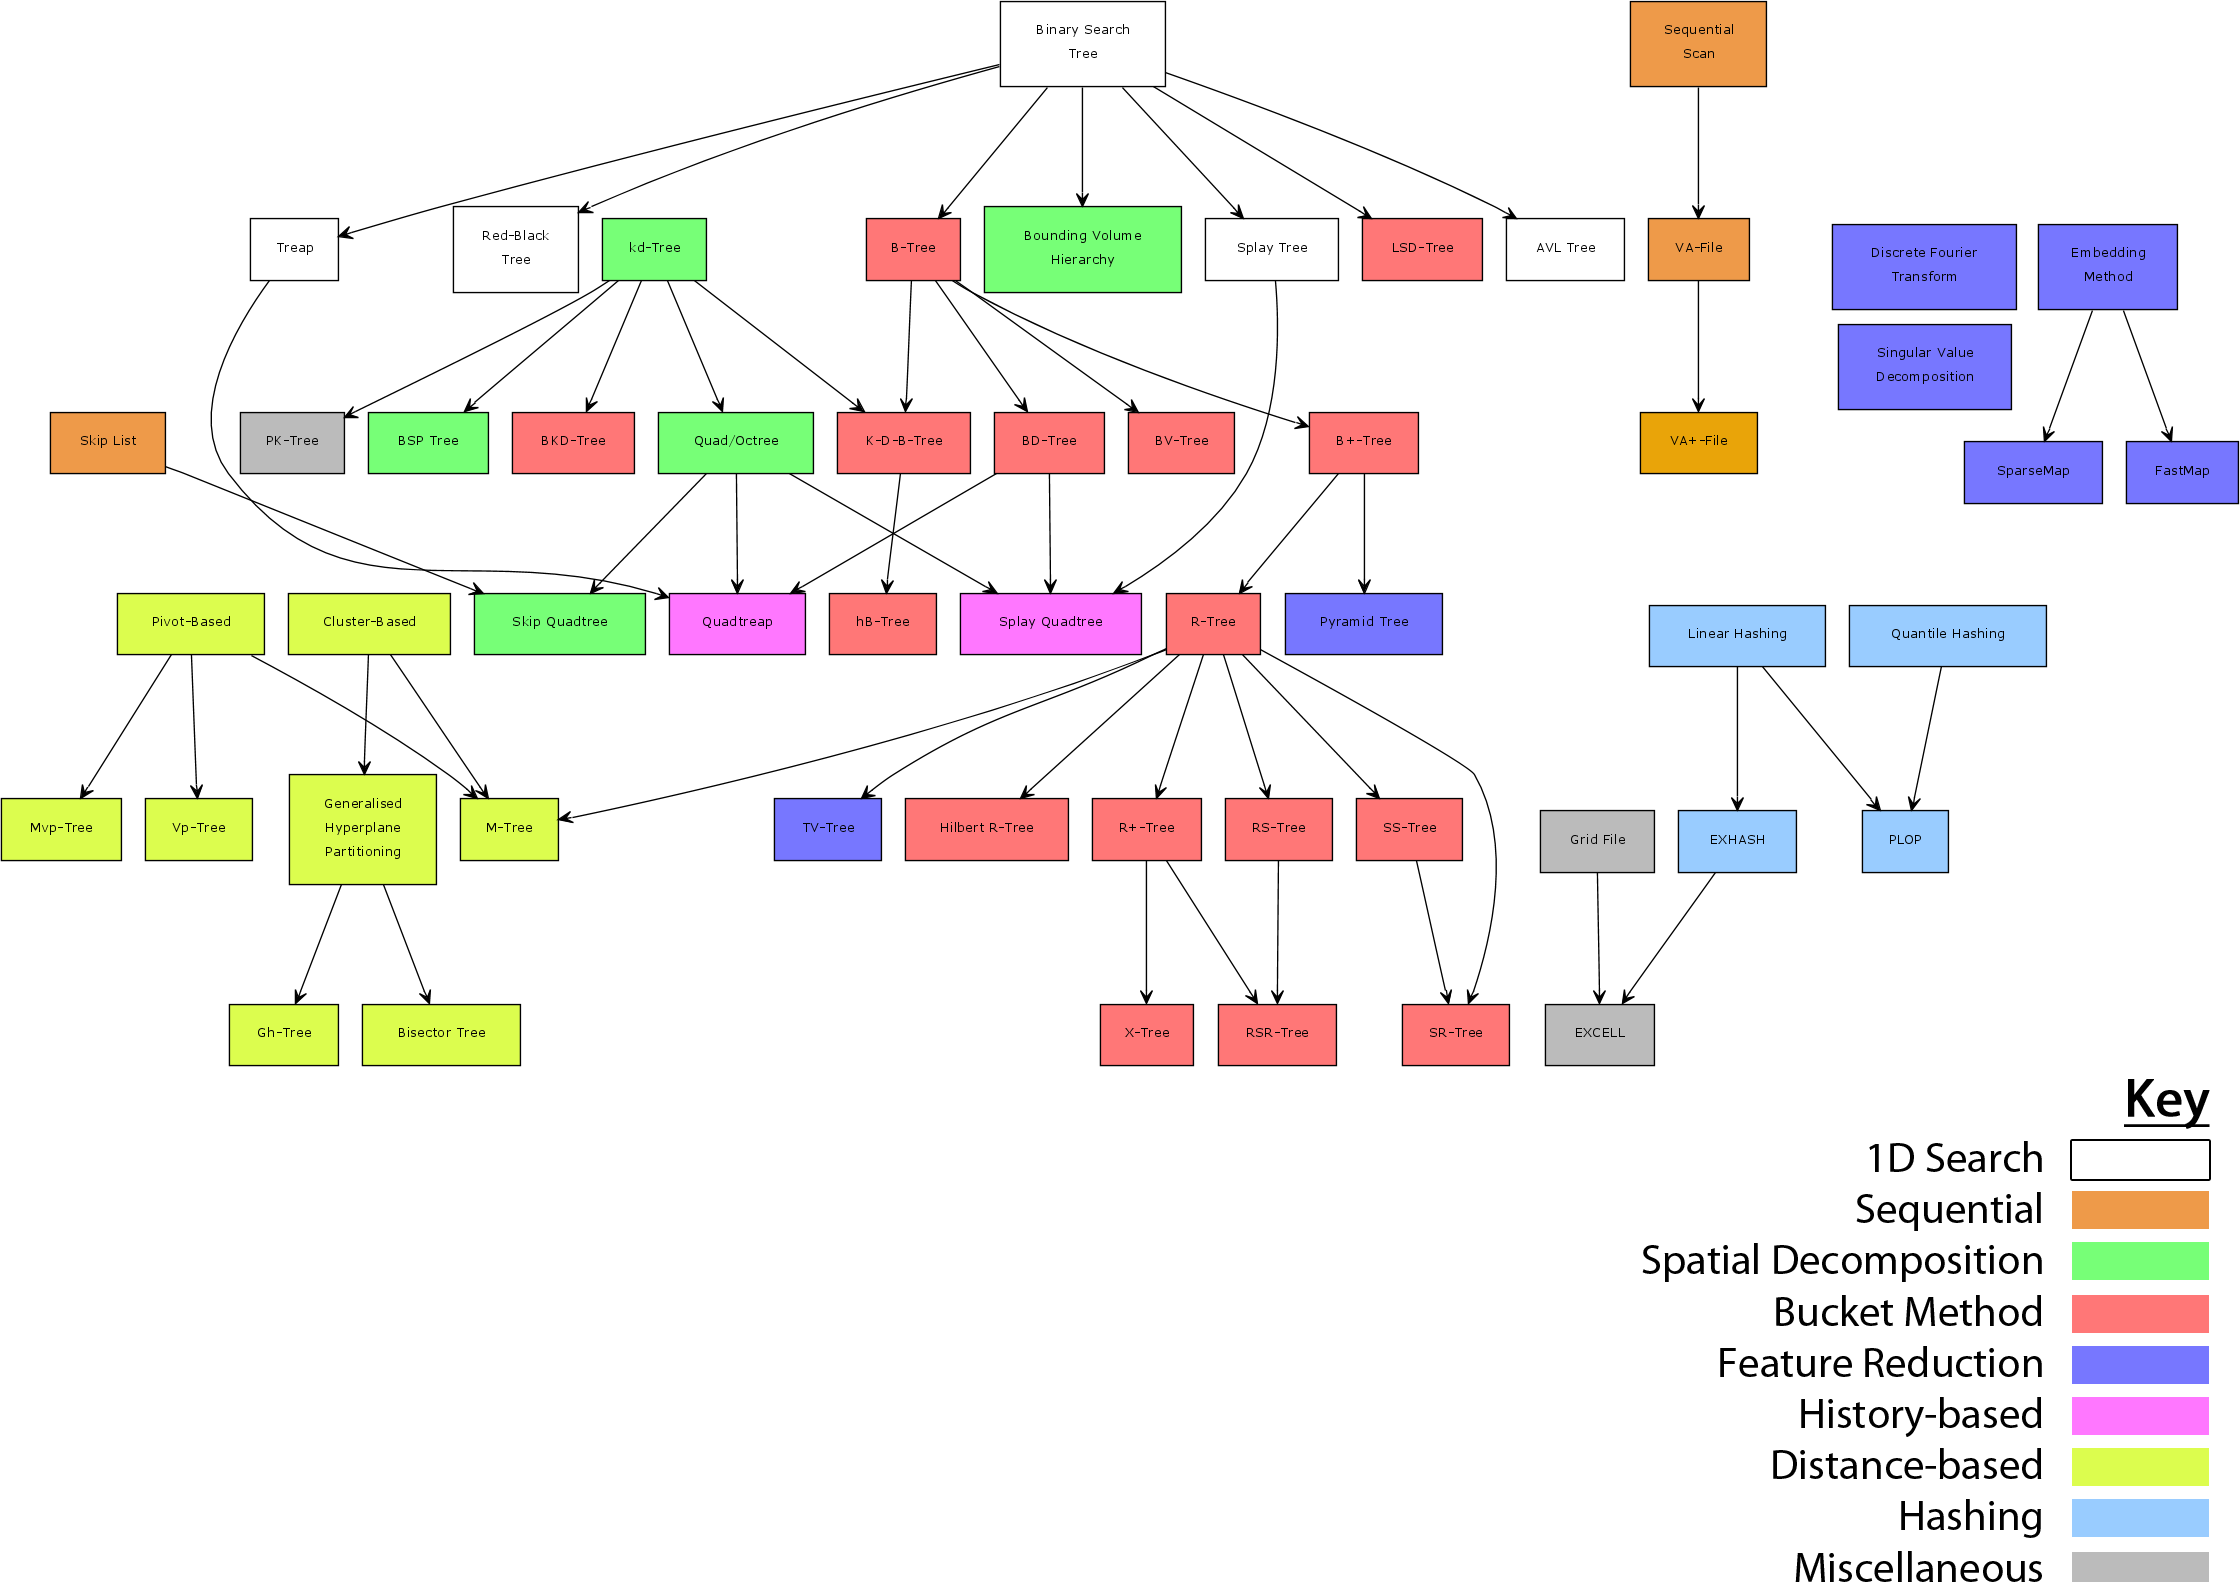
\includegraphics[scale=0.35]{figures/md_structure_taxonomy.png}
		\caption{Multi-dimensional Search Structure Taxonomy}
		\label{fig:structure-taxonomy}
	\end{figure}
\let \newpage \snewpage
\vfill 
\break % page break

	\newpage

\null  % Empty line
\nointerlineskip  % No skip for prev line
\vfill
\let\snewpage \newpage
\let\newpage \relax
	\begin{figure}[H]
		\centering
		\centerline{ 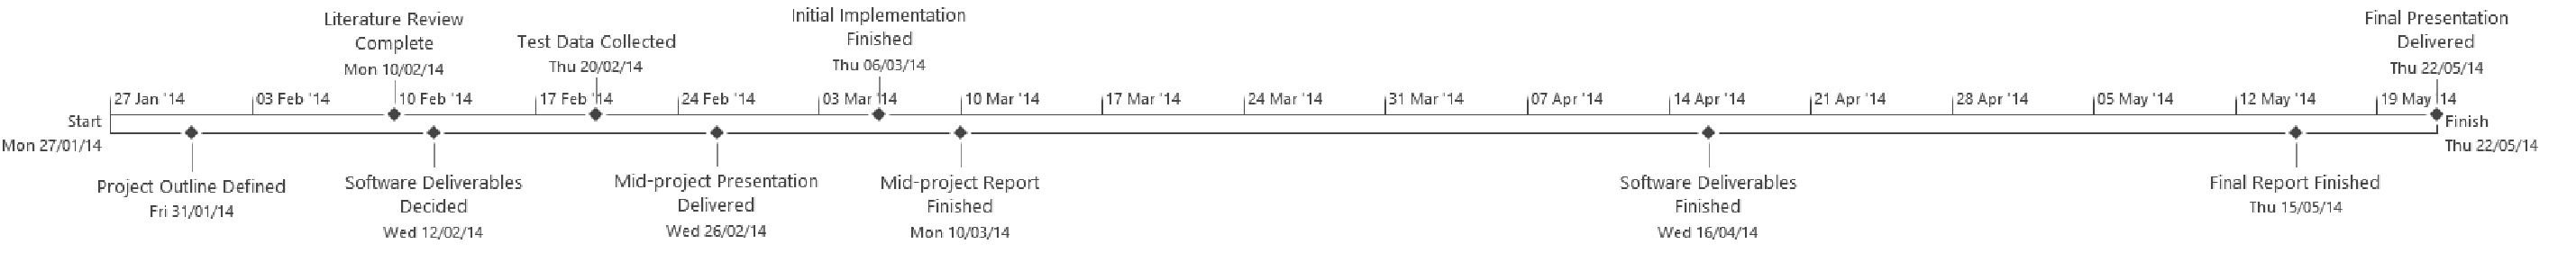
\includegraphics[scale=0.5]{figures/initial_schedule_timeline.pdf} }
		\caption{Initial Milestone Timeline Created on 20/02/14}
		\label{fig:initial-milestone-timeline}
	\end{figure}

	\begin{figure}[H]
		\centering
		\centerline{ 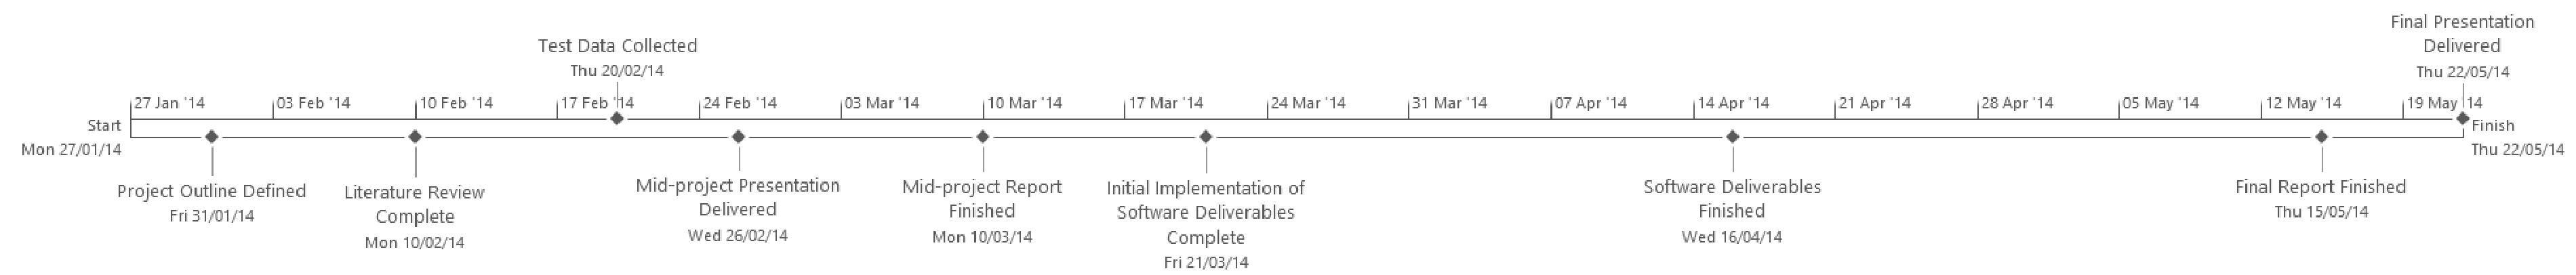
\includegraphics[scale=0.37]{figures/revised_schedule_timeline.pdf} }
		\caption{Revised Milestone Timeline Created on 20/02/14}
		\label{fig:revised-milestone-timeline}
	\end{figure}	
\let \newpage \snewpage
\vfill 
\break % page break

\end{landscape}

\begin{table}
	\centering
	\begin{tabular}{|p{2.8cm}|p{2.3cm}|p{3cm}|p{3cm}|p{3.5cm}|p{2cm}|}
		\hline
		\textbf{Index Structure} &
		\textbf{Memory Overhead} &
		\textbf{Bucket Method?} &
		\textbf{High-Dimensional Data} &
		\textbf{Complexity} \\
		\hline
		Sequential Scan & Low & No (but since data is stored contiguously, there are minimal I/O operations due to sequential access) & Often better than other structures with high $d$ (but significantly poorer performance with low $d$) & Low \\		
		B${}^{+}$-Tree & Low & Yes & One-dimensional & Low \\
		R-Tree & Moderate & Yes & Poor for $d > 10$ \cite{pyramid-tree} & Moderate \\
		Quadtree & Low with uniformly distributed data, high for skewed data due to unnecessary nodes caused by splitting sparse regions of data space & No & Poor because it tries to use balanced splits \cite{pyramid-tree} & Low \\
		Pyramid Tree & Low & Yes (based on B${}^{+}$-tree) & Good & High \\
		PK-Tree & Moderate & No (but uses similar method to reduce I/O operations) & Good & High \\
		Skip Quadtree & Moderate & No & Untested & Moderate \\
		Quadtreap & Low & No & Untested & Moderate \\
		Splay Quadtree & Moderate & No & Untested & Moderate \\
		\hline
	\end{tabular}
	\caption{Comparison of Dynamic Multi-Dimensional Structures}
	\label{tab:comparison}
\end{table}



\end{document}
